\documentclass[a4paper,10pt]{article}
%\documentclass[a4paper,10pt]{scrartcl}

\usepackage[utf8]{inputenc}
\usepackage{graphicx}
\usepackage{geometry}
\usepackage{wrapfig}
\usepackage{hyperref}
\graphicspath{ {./assets/} }
\hypersetup{
    colorlinks=true,
    linkcolor=blue,
    filecolor=magenta,
    urlcolor=cyan,
    }
\geometry{
 a4paper,
 total={170mm,257mm},
 left=20mm,
 top=20mm,
 }

\title{Le manuel d'utilisation de mon moteur de jeu}
\author{DERRUAU Noam}
\date{25/10/2023}

\pdfinfo{%
  /Title    (Le manuel d'utilisation de mon moteur de jeu)
  /Author   (DERRUAU Noam)
}

\begin{document}
\maketitle

\newpage
\tableofcontents
\newpage

\section{OpenGL}

\subsection{Qu'est ce qu'OpenGL?}

OpenGL est une API graphique dont les fonctionnalités sont spécifiés (mais non codés) par le groupe \href{https://www.khronos.org/}{Khronos}. L'implémentation des fonctions est quand à elle laissée aux fabriquants de cartes graphiques (Nvidia, AMD, Intel, etc...). Les librairies utilisés en interne par l'ordinateur sont donc dépendentes de notre matériel.
Pour mon moteur de jeu, j'utiliserais OpenGL 3.3, aussi appelé Modern OpenGL
\\
\begin{wrapfigure}{r}{0.5\textwidth}
    \centering
    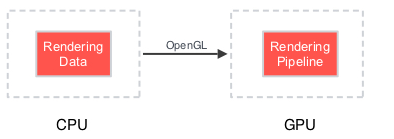
\includegraphics[width=0.5\textwidth]{OpenGL_purpose}
\end{wrapfigure}

Le principe d'OpenGL est d'être une passerelle entre le Processeur et la Carte Graphique, il ne s'occupe pas de la logique de l'application, mais il apporte une couche d'abstraction lors du rendu sur écran.
\\
Pour bien comprendre l'API, il est essentiel d'être au point sur le mode de fonctionnement d'une carte graphique ainsi que certains autres concepts détaillés ci-après.

\subsection{Concepts de base}
\subsubsection{La carte graphique}
Une carte graphique est un composant de l'ordinateur, au même titre que le processeur, dont le but est de transformer des données graphiques envoyés par le processeur en une image cohérente sur un écran. Un processeur est capable d'accomplir cette tache sans l'aide d'une carte graphique, cependant l'opération est très lente et nécessite beaucoup d'optimisation pour tourner avec un nombre d'images par seconde acceptable.

\paragraph{Différence entre un processeur et carte graphique}
\begin{wrapfigure}{l}{0.5\textwidth}
    \centering
    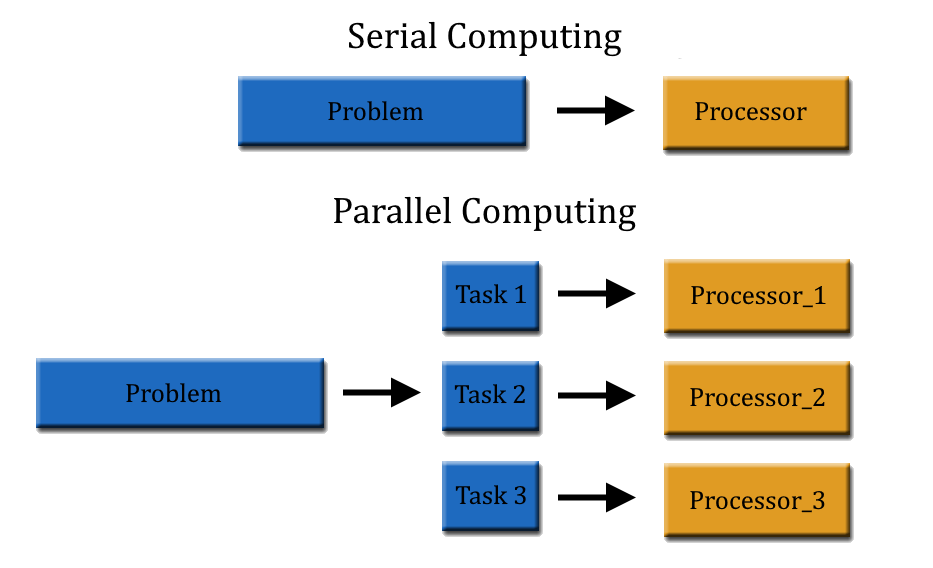
\includegraphics[width=0.5\textwidth]{parallel_computing_vs_sequential_computing}
\end{wrapfigure}
Un processeur moderne va peut être avoir 8 où 16 coeurs qui effectuent autour de 3.5 milliards d'opérations par seconde. Ces coeurs ne sont pas spécialisés, c'est à dire qu'ils peuvent effectuer n'importe quel type de calcul mais ceux-ci sont fait séquentiellement (les uns après les autres).
Une carte graphique moderne va quant à elle avoir autour de 1000 coeurs spécialisés qui effectuent environ 1 millard d'opérations par seconde. Elle excèle lorsque les taches qui lui sont donnés sont faisables en parallèle, c'est à dire que tout les coeurs peuvent travailler sur des petites parties indépendantes et similaires de ladite tache. Le rendu d'image où d'espaces 3D est justement une tache parallélisable, c'est pour cela que le processeur laisse généralement ce travail à la carte graphique

\paragraph{RAM et VRAM}
La mémoire vive (RAM) est un type de mémoire qui permet un accès très rapide aux données, ainsi lorsque vous créez où modifiez une variable dans un programme, celle ci est stockée dans la RAM (on part du principe qu'il n'y a pas de cache) et non sur votre disque dur dont la vitesse d'accès à l'information est 1 million de fois plus lente que sur la RAM. Ainsi rajouter de la RAM vous permettra de stocker plus de données en accès rapide. Cependant, si votre carte graphique a du mal à stocker toutes les données graphiques qu'on lui envoie, rajouter de la RAM ne remédiera pas au problème. Les cartes graphiques possèdes des unités de RAM dédiés et isolés du processeur, appelés VRAM (Video Random Access Memory) directement intégrés à la carte graphique, donc de taille immuable.

\paragraph{Communication entre un processeur et une carte graphique}
La communication entre le processeur et la carte graphique s'effectue au travers d'un cable PCI-Express, qu'on appelle un bus qui possède une grande bande passante. Il n'est pas possible d'accéder directement à une information stockée dans la RAM depuis la carte graphique, ainsi pour afficher un objet 3D à l'écran, il faut d'abord copier cet objet dans la VRAM. De plus, il vaut mieux charger à l'avance dans la VRAM toutes les données que l'on souhaite utiliser, car la communication au travers du bus est très lente. Ce problème est une limitation physique, et donc irrémédiable. En effet, puisque le bus fait aux alentours des $d = 10cm$ de long et que 1 bit d'information traverse le bus à la vitesse de la lumière $c$, on met $t_b = \frac{d}{c}=0.25ns$ pour envoyer un bit. De plus, un seul bit d'information est envoyé par cycle du processeur, donc pour un processeur à $c_s = 4GHz$ qui envoie $i=1Mo$ d'information à la carte graphique, on met $\Delta t = (t_b + \frac{2}{c_s})i = 6.4ms$, ce qui est très lent.

\paragraph{Comment faire un programme qui tourne sur la carte graphique}
Les programmes qui tournent sur la carte graphique sont appelés des shaders. Dans OpenGL, il en existe plusieurs type qui s'exécutent dans cet ordre:
\begin{enumerate}
 \item Le Vertex Shader: il prend en entrée des données quelconques (généralement un point et quelques informations à propos de celui-ci) et retourne une nouvelle position de ce point. À la fin de ce processus le shader forme les \hyperref[subsubsec:Primitives]{primitives} associés à ces points. Les primitives sont les formes de bases associés à des points, par exemple 2 points forment une ligne, 3 points un triangles, etc... On choisit au préalable à quel type de primitives correspondent nos points. Le vertex shader ne mixe pas plusieurs types de primitives.
 \item Le Tesselation Control Shader et Tesselation Evaluation Shader: s'occupe de subdiviser les primitives de base pour lui ajouter des détails tout en interpolants les valeurs supplémentaires associés au point. Les primitives issues de la subdivision sont de même types que la primitive de départ. La subdivision est inscrite dans la primitive de départ, donc cela ne change pas ses contours.
 \item Le Geometry Shader: il prend en entrée une primitive, et permet de retourner une ou plusieurs primitives, dont le type peut être différent.
 \item Le Fragment Shader: Juste après le Geometry Shader se produit l'étape de \href{https://fr.wikipedia.org/wiki/Rast\%C3\%A9risation}{Rastérisation} qui convertit la géométrie en pixels. Après cette étape vient le Fragment Shader. Il permet de définir une couleur pour chacun des pixels issu du Raster. Finalement tout les objets de l'environnement sont placés à leur position respective et l'image finale est créée, c'est l'étape de Color Blending.
 \item Compute Shader: Un programme totalement déconnecté du procédé de rendu graphique, utilisé pour calculer des informations générales de manière parallèle.
\end{enumerate}


\begin{figure}[h]
    \centering
    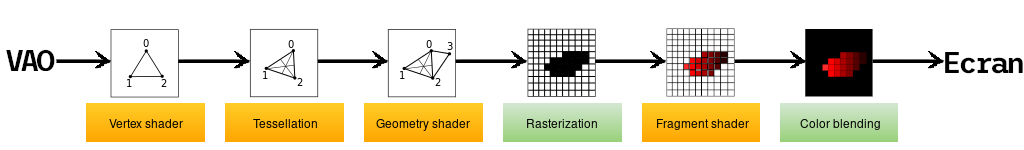
\includegraphics[width=1\textwidth]{shader_pipeline_sideways}
    \caption{Chaine d'éxécution des shaders}
\end{figure}

\paragraph{Les choses à éviter lorsqu'on écrit des shaders} De pars la nature parallèle des shaders, il est déconseillé de faire des programmes qui branchent (if else). En effet, imaginons un programme qui contienne un branchement et que l'une de ses branches mène à un algorithme qui prends beaucoup plus de temps à calculer que celui de l'autre branche. Si sur 100 exécutions du shader, seule une seule valeur prend la branche longue, tout le programme devra attendre que cette branche finisse de s'éxecuter pour renvoyer le résultat final.

\subsubsection{Buffers}
Dans OpenGL, un buffer est une région continue de VRAM qui contient des informations non typés, par exemple cela veut dire qu'on ne dispose d'aucun moyen pour savoir si 01000001 représente le caractère A en ASCII où juste le nombre 65.
Les buffers peuvent soient être mutables soit non-mutables. Ce qu'on veut dire par là, c'est que la taille des buffers et leurs emplacement mémoire n'est pas mutable, mais leur contenu lui l'est. Les buffers non-mutables ouvrent la porte à des optimisations, non détaillés ici.

\newpage
\subsubsection{Primitives}
\label{subsubsec:Primitives}
Les primitives sont les différents moyens de représenter une suite de points. On peut par exemple dire que la liste $(p_0, ..., p_n)$ représente juste des points de l'espace, mais aussi une suite de segments $[p_ip_{i+1}], \forall i \in  [\![0;n-1]\!]$ ou encore une liste de triangles dont les points $(p_i, p_{i+1}, p_{i+2}), \forall i \in  [\![0;n-2]\!]$ sont les sommets. Dans OpenGL, les primitives disponibles sont les suivantes:

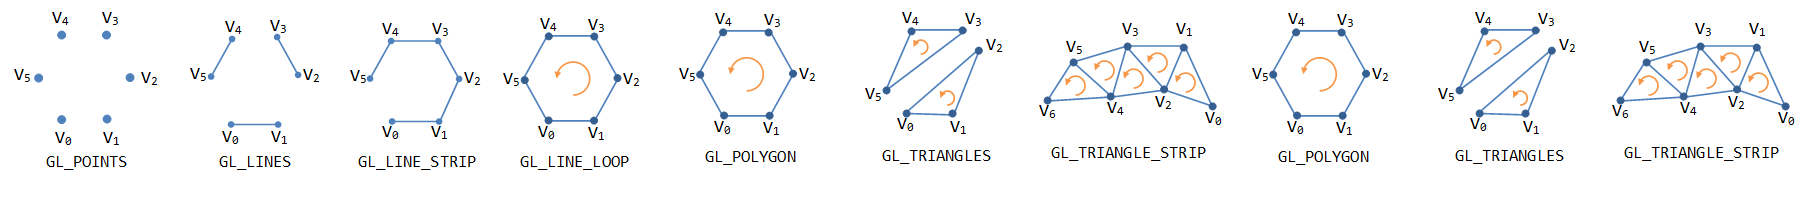
\includegraphics[width=0.96\textwidth]{OpenGL_primitives_flattened}

Notez que les Quads ne sont plus disponibles puisque la surface que les points délimitée est ambiguë. En effet, si les 4 points ne sont pas dans le même plan, quels points font partie de la surface?

\subsubsection{Textures}
[WORK IN PROGRESS]

\subsection{Fonctionnement interne d'OpenGL}
[WORK IN PROGRESS]

\subsection{Plus de renseignements}
Ce manuel n'est pas une documentation de la spécification OpenGL 3.3, aussi je ne détaillerais pas plus son fonctionnement. Pour approfondir vos connaissances, je conseille de lire les wikis suivants:
\begin{itemize}
 \item \href{https://www.khronos.org/opengl/wiki/}{Le wiki OpenGL de Khronos}: il permet de comprendre les concepts spécifiques à la libraire et les différents systèmes interagissent entre eux.
 \item \href{http://www.hyzgame.org.cn/OpenGL/man3/bottom.php}{La référence des fonctions OpenGL 3.3}: Contient une liste exhaustive de toutes les fonctions d'OpenGL 3.3 ainsi que comment les utiliser.
 \item \href{https://learnopengl.com}{LearnOpenGL.com}: Un site qui permet d'apprendre les concepts de rendu d'espace 3D avec OpenGL. Il est conseillé d'avoir lu le Wiki de Khronos avant de lire le contenu de ce site
 \item \href{https://www.youtube.com/playlist?list=PLn3eTxaOtL2PDnEVNwOgZFm5xYPr4dUoR}{OpenGL avec Python}: une série de vidéos qui explique comment utiliser OpenGL sous python (utile dans le cadre de ce projet)
\end{itemize}


\section{Structure du moteur de jeu}

\subsection{But à accomplir}
Ce moteur de jeu est créé dans le but d'y faire tourner une simulation de fluide en 3D en temps réel.
Je ne détaillerais pas ici les fonctionnalités que je souhaite avoir dans ma simulation, mais seulement ce que le moteur de jeu doit être capable de faire seul.
\begin{itemize}
 \item On doit pouvoir se mouvoir dans un espace 3D avec une caméra à la première personne.
 \item On doit pouvoir changer de niveaux.
 \item Chaque niveau peut être composé d'une multitude d'entités, chacune associée à son draw call et sans occlusion culling.
 \item Le système de déplacement est composé de 2 modes. Un mode déplacement dans lequel on peut se mouvoir mais pas interagir avec les entités du niveau. Un autre mode, appelé mode interraction dans lequel on ne peut se mouvoir ni bouger l'orientation de la caméra mais on peut interragir avec le monde en cliquant sur les entités affichés à l'écran.
\end{itemize}


\subsection{Choix du langage}

Puisque ce projet a vocation à être un \href{https://www.scei-concours.fr/tipe.php}{TIPE}, la priorité dans le choix du langage va être la verbosité de sa syntaxe. Le langage choisi doit être simple à lire et à comprendre pour les examinateurs qui vont juger le TIPE. De plus, le langage choisi doit pouvoir tourner sur les ordinateurs du lycée sans installer de logiciels supplémentaires. (Cela me limite au Python, Ocaml et Javascript)

C'est pour cela que je m'oriente vers le Python.
En tant que professeurs de Mathématiques et de Physique, ils ont surement de l'expérience avec ce langage et sa syntaxe non verbose est parfaite pour rapidement comprendre le fonctionnement de mes algorithmes.

On peut critiquer ce choix, notamment car une simulation de fluide en temps réel nécessite beaucoup de calculs et Python n'est pas le plus rapide des langages, mais je n'ai pas encore assez d'expérience avec Ocaml pour me lancer dans ce genre de projet et les examinateurs n'ont probablement jamais touchés à du Javascript.

\subsection{Composants principaux du moteur de jeu}
[WORK IN PROGRESS]

\subsubsection{Le Rendering Engine}

\end{document}
